\problemname{Inflation}
People in southern Sweden are known to eat falafel a lot. The price of falafel is highly volatile, 
and the best way to analyze the state of the economy is to go to the same falafel place every 
day and add up all the prices on their menu.

A falafel place has $N$ different dishes on their menu. The $i$th dish has price $p_i$. 

Every day,
one of the following events happen:

\begin{enumerate}
    \item \verb|INFLATION x|: The integer $x$ is added to all prices.
    \item \verb|SET x y|: Every dish with price $x$ gets its price set to $y$.
\end{enumerate}

Your task is to process $Q$ days, and after each day print the sum of all prices $p_i$.

\section*{Input}
The first line contains one integer $N$, the number of dishes.

The second line contains $N$ integers $p_1, p_2, \ldots, p_N$.

The third line contains one integer $Q$, the number of days.

The following $Q$ lines each contain a string $s$ followed by either one or two integers. 

If $s$ is \verb|INFLATION|, then one integer $x$ follows. This means that $x$ is added to all prices
on this day.

If $s$ is \verb|SET|, then two integers $x$ and  $y$ follow. This means that all dishes with price $x$ get
their price set to $y$ on this day.


\section*{Output}
Print $Q$ lines, the sum of all prices $p_i$ after each day.

\section*{Constraints and Scoring}

\noindent
\begin{itemize}
  \item $1 \leq N \leq 3 \cdot 10^5$.
  \item $1 \leq p_i \leq 10^6$ (for each $i$ such that $1 \leq i \leq N$).
  \item $1 \leq Q \leq 10^5$.
  \item $1 \leq x,y \leq 10^6$ for all days. 
\end{itemize}

\noindent
\textbf{Note}: The answer may not fit in a $32$-bit integer, so be aware of overflows if you are using C++.

Your solution will be tested on a set of test groups, each worth a number of points. 
Each test group contains a set of test cases. To get the points for a test group you need to 
solve all test cases in the test group.

\noindent
\begin{tabular}{| l | l | l |}
\hline
Group & Score & Limits \\ \hline
  1      & 14      & $N=1$\\ \hline
  2      & 28      & $N, Q, p_i, x, y \leq 100$  \\ \hline
  3      & 19      & There are only \verb|INFLATION| events  \\ \hline
  4      & 23      & There are only \verb|SET| events  \\ \hline
  5      & 16      & No additional constraints  \\ \hline
\end{tabular}

\section*{Example}

This figure corresponds to the first two days of sample $1$. Note that the sum of prices after the
first day is $16$, so the first integer in the output is $16$.
\begin{figure}[h]
  \centering
  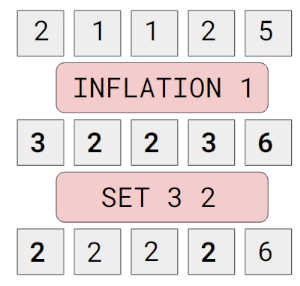
\includegraphics{inflation-sample-2.png}
\end{figure}
